% Copy paper_figures_v1/ beside the paper main file, or adjust the paths.
% Requires graphicx, booktabs, and a Chinese-capable document class (e.g. ctex).
% These snippets have not been compiled against the user's thesis template.

\begin{figure}[htbp]
  \centering
  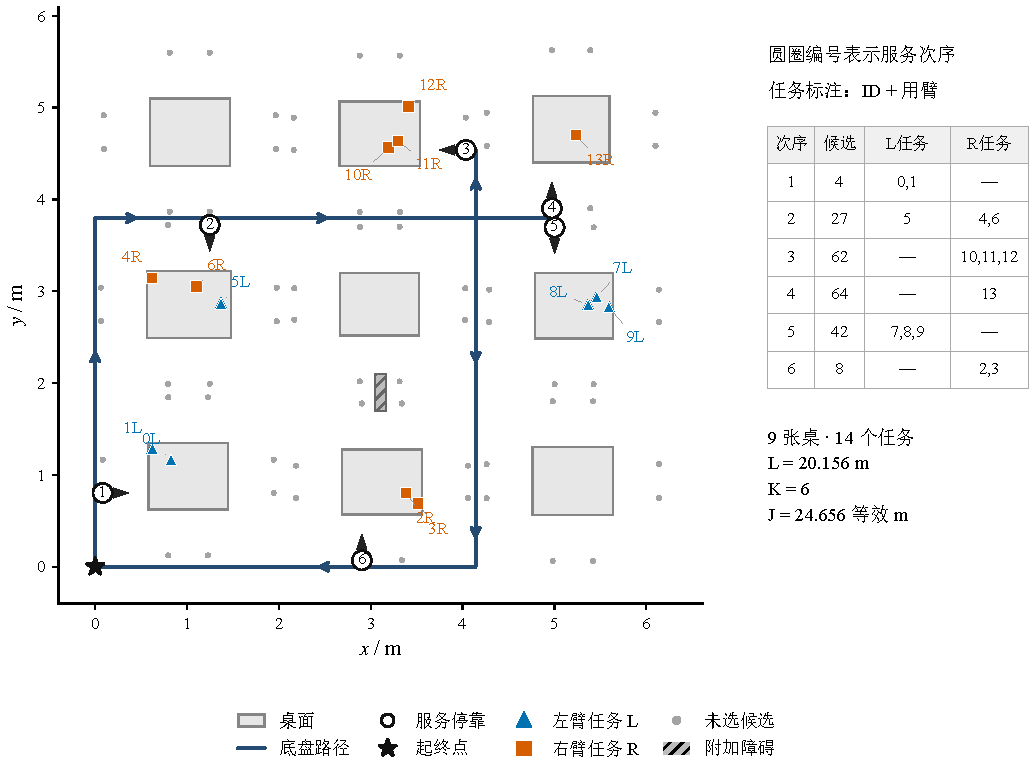
\includegraphics[width=0.95\textwidth]{paper_figures_v1/fig1_scene.pdf}
  \caption{二维静态桌面任务的完整输出示例（seed=771903）：9张桌、14项任务、72个候选，最终采用6次停靠。三角形和方形分别表示左、右臂任务；任务ID从0开始，空心圆编号为服务次序。黑箭头表示停靠朝向，蓝线及箭头表示保存底盘路径；细灰引线仅对应文字标注，星号为起终点。右表列出任务分配。$L=20.156$ m，$K=6$，$J=L+0.75K=24.656$等效m。该图是代理约束下的格式与几何示例，不是实测任务时间或真实机械臂执行证据。}
  \label{fig:rc3-scene-output}
\end{figure}

\begin{figure}[htbp]
  \centering
  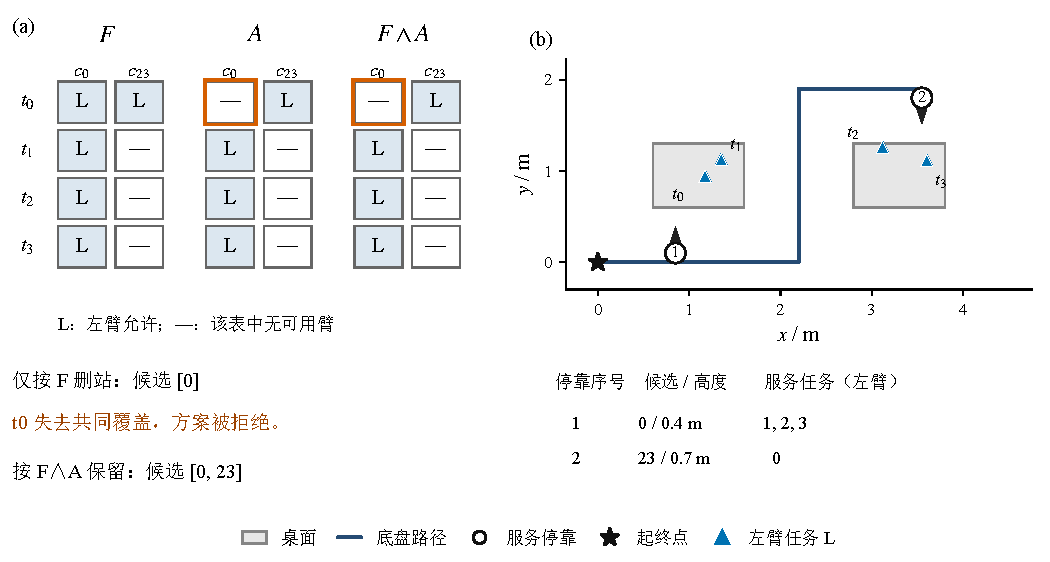
\includegraphics[width=0.95\textwidth]{paper_figures_v1/fig2_constraints.pdf}
  \caption{共同约束贯穿路线规范化的必要性：2桌4任务的合成反例（seed=870001）。(a)展示所选候选$c_0,c_{23}$的$F,A,F\cap A$；L表示允许左臂，横线表示无可用臂。仅按$F$删除$c_{23}$后，$t_0$失去共同覆盖；共同约束保留两站。(b)只绘制保存的成功完整路径，未将失败方案绘制为认证路径。$L=11.3$ m，$K=2$，$J=12.8$等效m。可达表与跨桌分配为刻意构造，不表示真实工作空间或臂轨迹。}
  \label{fig:rc3-common-constraint}
\end{figure}

\begin{figure}[p]
  \centering
  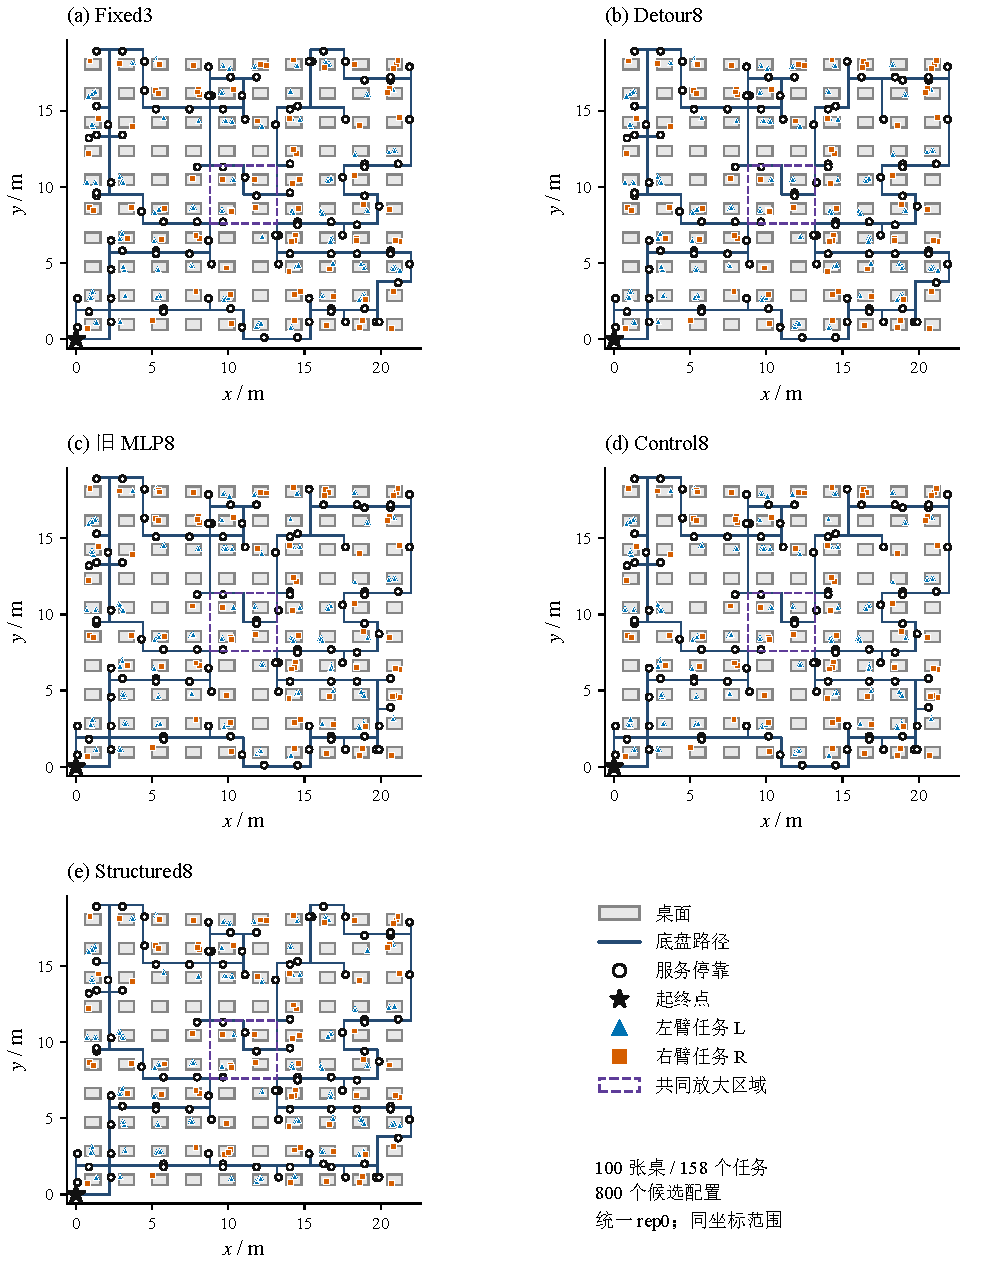
\includegraphics[width=0.95\textwidth,height=0.82\textheight,keepaspectratio]{paper_figures_v1/fig3_routes100.pdf}
  \caption{原列表首个百桌场景的五方法保存路线（seed=1565649625，158任务、800候选，统一rep0）。Fixed3为无修复初始参照，其余方法固定8次修复，未混入400 ms软预算实验。五面板同轴同符号；虚线框为导航包络各方向中央20\%。成本见表\ref{tab:fixed-main100-costs}；本例Structured8的$J=277.8$高于Detour8的276.2，单例不替代整体统计结论。$J=L+0.75K$为等效路程成本，不是总服务耗时。}
  \label{fig:rc3-main100-routes}
\end{figure}

\begin{figure}[p]
  \centering
  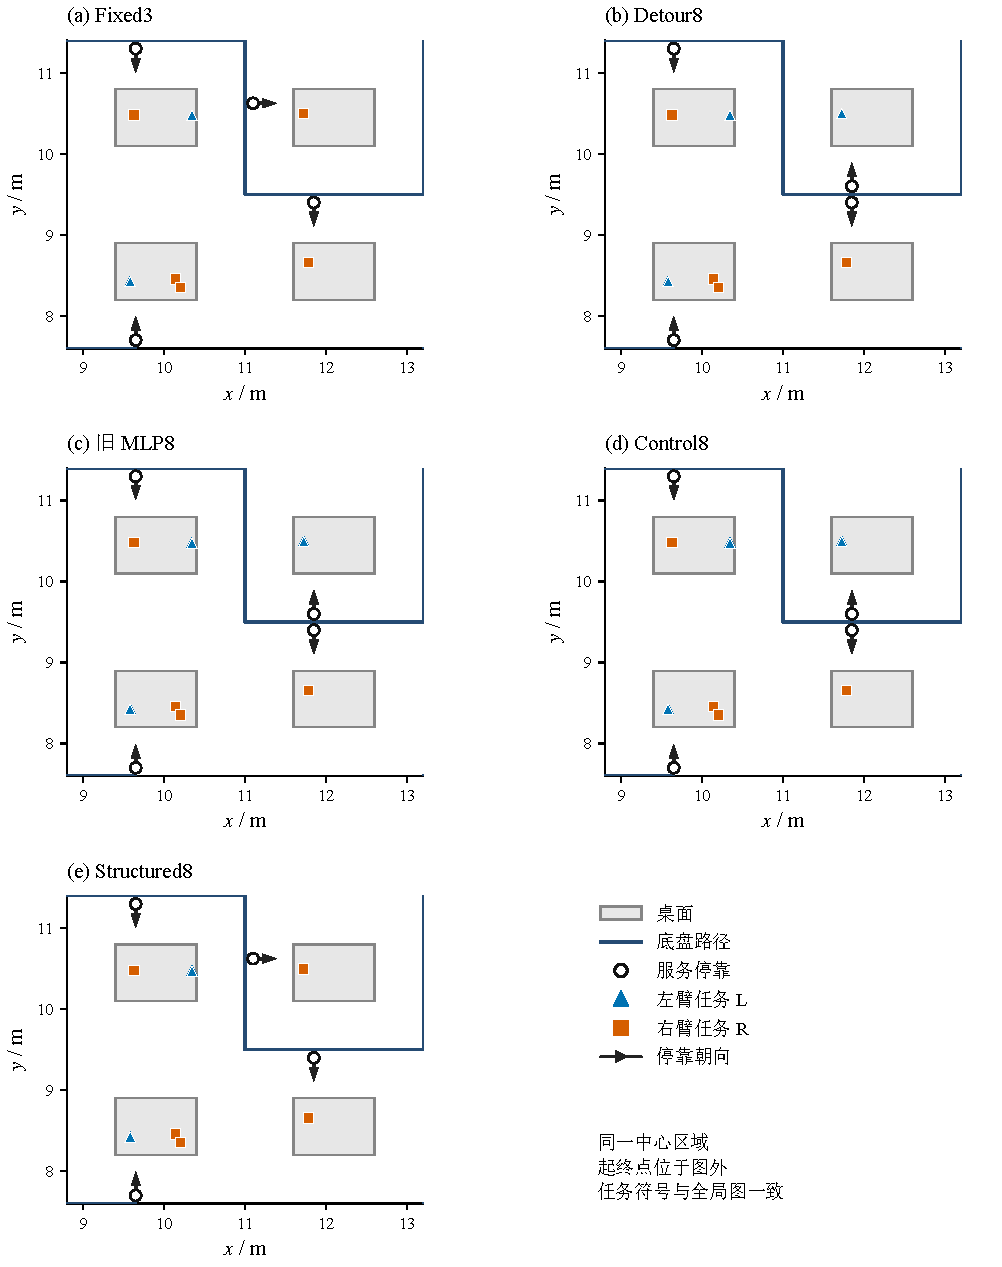
\includegraphics[width=0.95\textwidth,height=0.82\textheight,keepaspectratio]{paper_figures_v1/fig3_zoom.pdf}
  \caption{图\ref{fig:rc3-main100-routes}的共同中心区域放大：$x\in[8.8,13.2]$ m，$y\in[7.6,11.4]$ m。裁剪按导航包络各方向中央20\%确定，不按模型收益或路线差异选择；面积约为整体包络4\%。黑箭头表示停靠朝向，起终点位于视窗外，边界处路线继续延伸。本图只解释保存方案的局部几何，不增加新样本、计时或物理验证。}
  \label{fig:rc3-main100-zoom}
\end{figure}

\begin{table}[htbp]
\centering
\caption{固定百桌场景的保存方案成本。种子1565649625，统一取rep0；Fixed3为无修复初始参照，其余方法采用固定8次修复。$J=L+0.75K$为等效路程成本。}
\label{tab:fixed-main100-costs}
\begin{tabular}{lrrrr}
\toprule
方法 & 修复预算 & $L$ / m & $K$ & $J$ / 等效 m \\
\midrule
Fixed3 & 0 & 209.550 & 94 & 280.050 \\
Detour8 & 8 & 205.700 & 94 & 276.200 \\
旧 MLP8 & 8 & 205.100 & 93 & 274.850 \\
Control8 & 8 & 205.100 & 93 & 274.850 \\
Structured8 & 8 & 207.300 & 94 & 277.800 \\
\bottomrule
\end{tabular}
\end{table}

